\begin{recipe}
[ %
        preparationtime = {\SIrange{3}{5}{\hour}},
        portion = {\portion{4--5}},
        source = {HeNine}
    ]{Goulash}

        \begin{figure}[p]
	        \centering
	        \makebox[\textwidth][c]{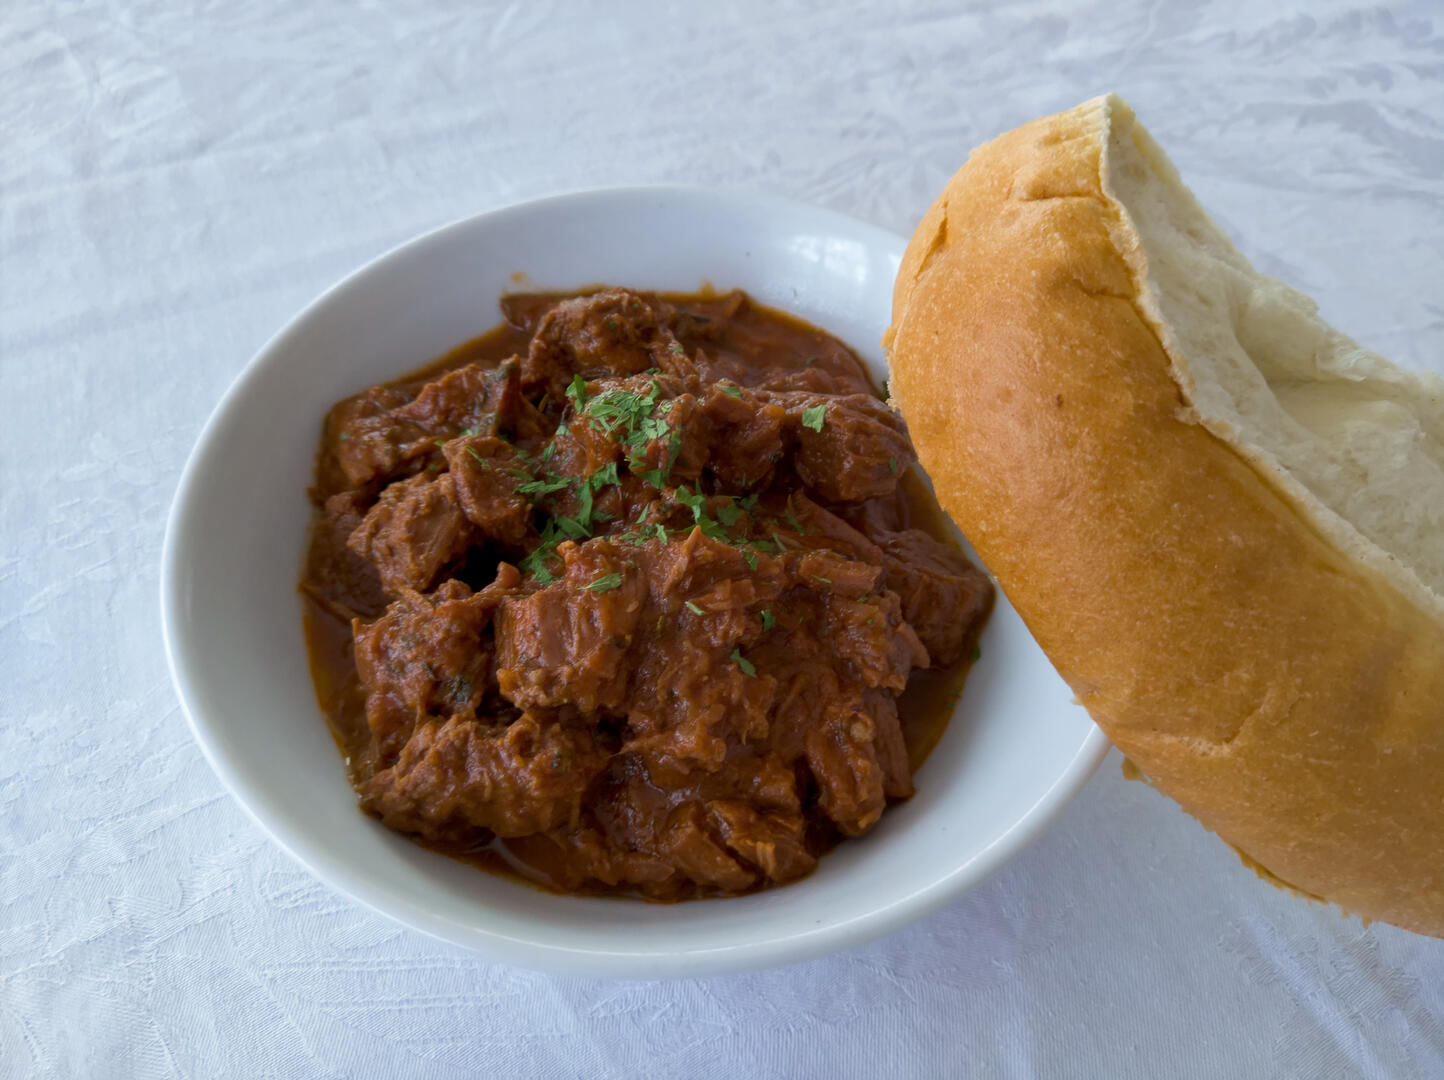
\includegraphics[height=\textheight]{goulash/IMG_20200202_120631.jpg}}
	    \end{figure}

	    \introduction{%
	        \textbf{\large BEEF}

	        Use a cheaper cut of meat, like thigh, flank or shoulder. You'll be stewing it to soften and adding lots of spices to maximize the taste.

            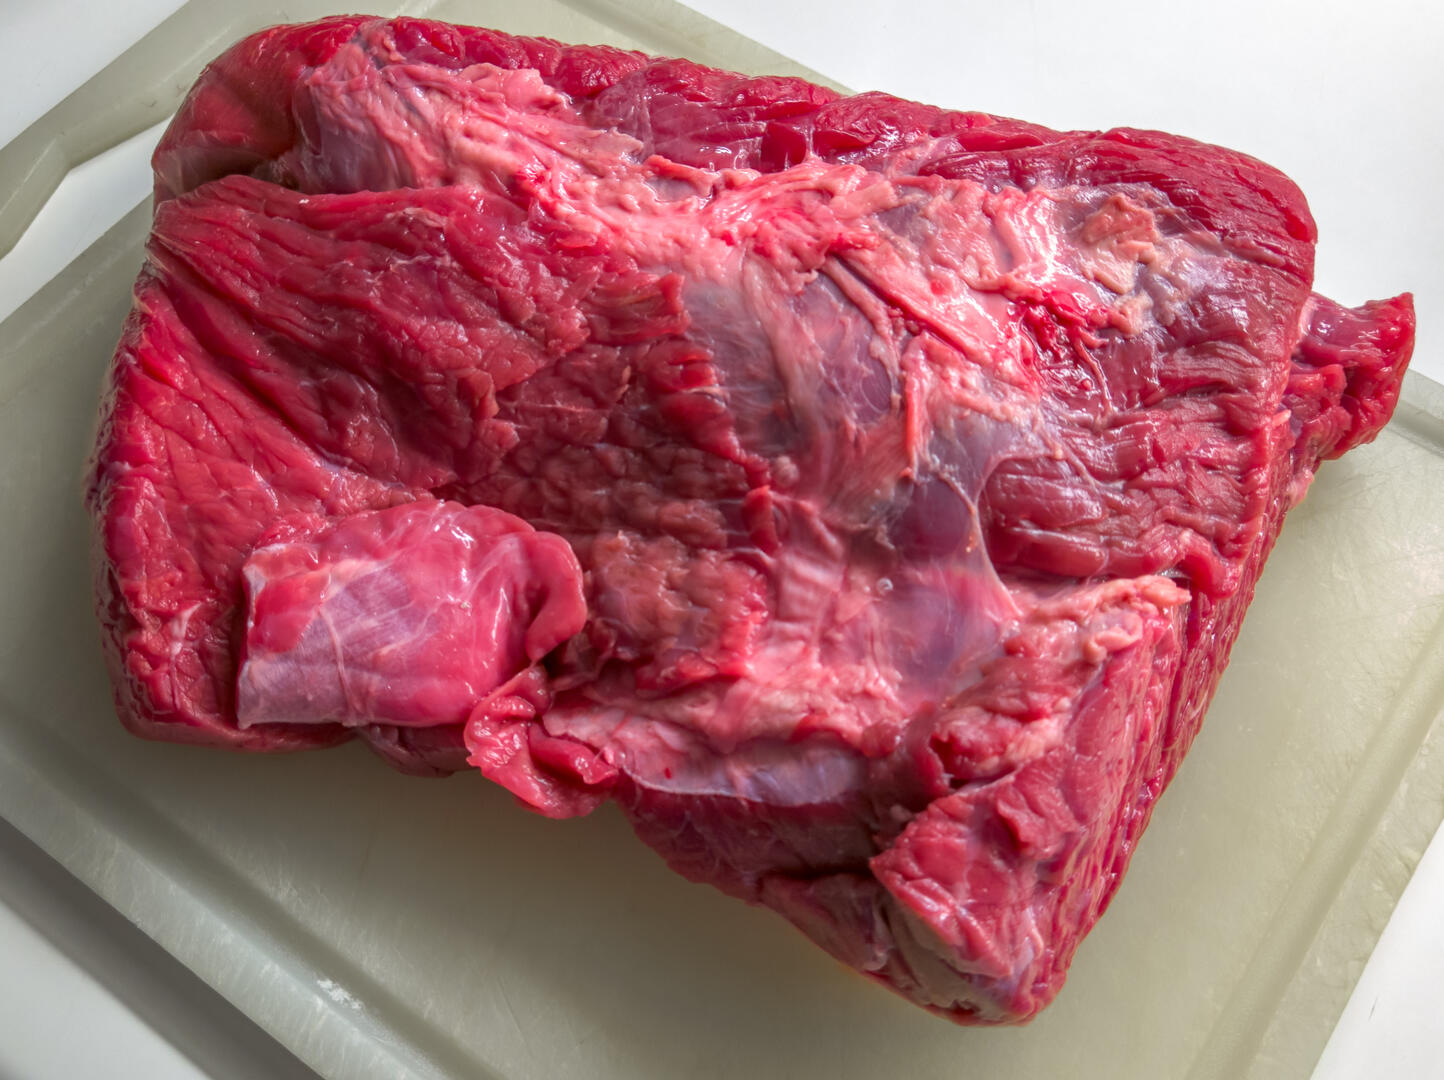
\includegraphics[width=\textwidth]{goulash/IMG_20200202_084818.jpg}

            \textbf{\large Onion}

            This is a pretty flexible recipe. You can use anywhere between 0.3 and 1.5 kg (per 1 kg of meat). I like a meatier version and onions make me farty.

            You can also use red or white or yellow onions OR A MIX! Fuck this boi up with onions!

            \newpage
            \textbf{\large Spice mix}

            The amounts here are eyeballed and I tend to go easy on cumin, but this mix works for me.

            Because we stew the meat for a long time I try to leave the herbs and spices in larger chunks: whole juniper berries, whole bay leaf, whole peppercorns, whole slightly crushed garlic cloves; I haven’t tried whole cumin and caraway, but that should also work.

            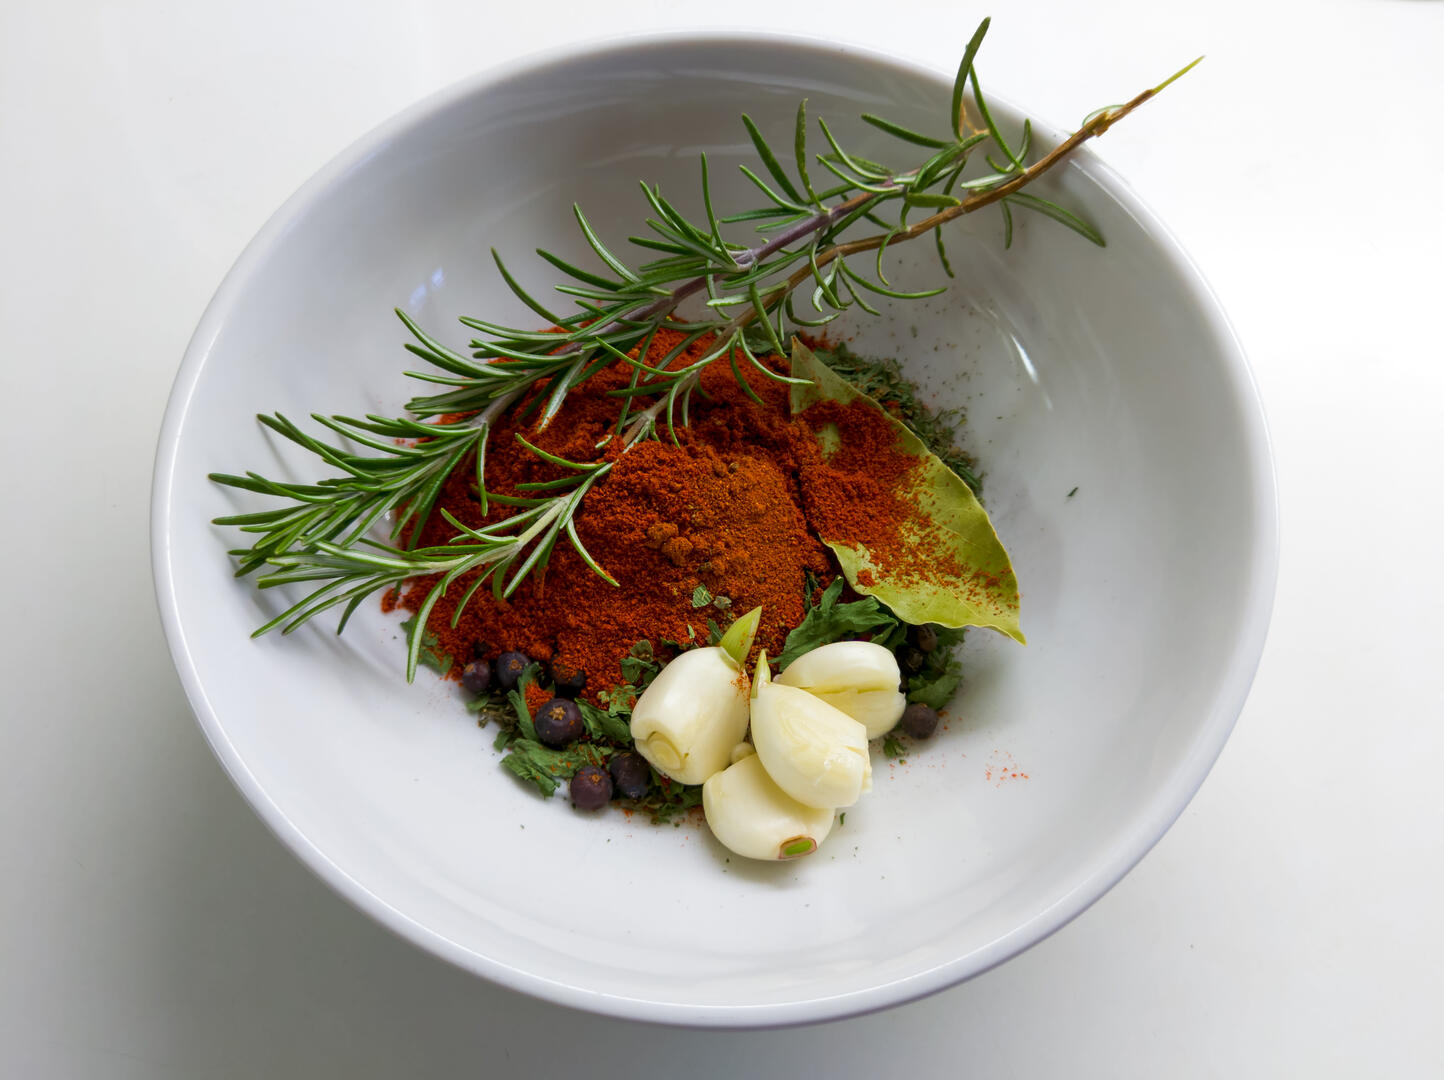
\includegraphics[width=0.5\textwidth]{goulash/IMG_20200202_095145.jpg}%
            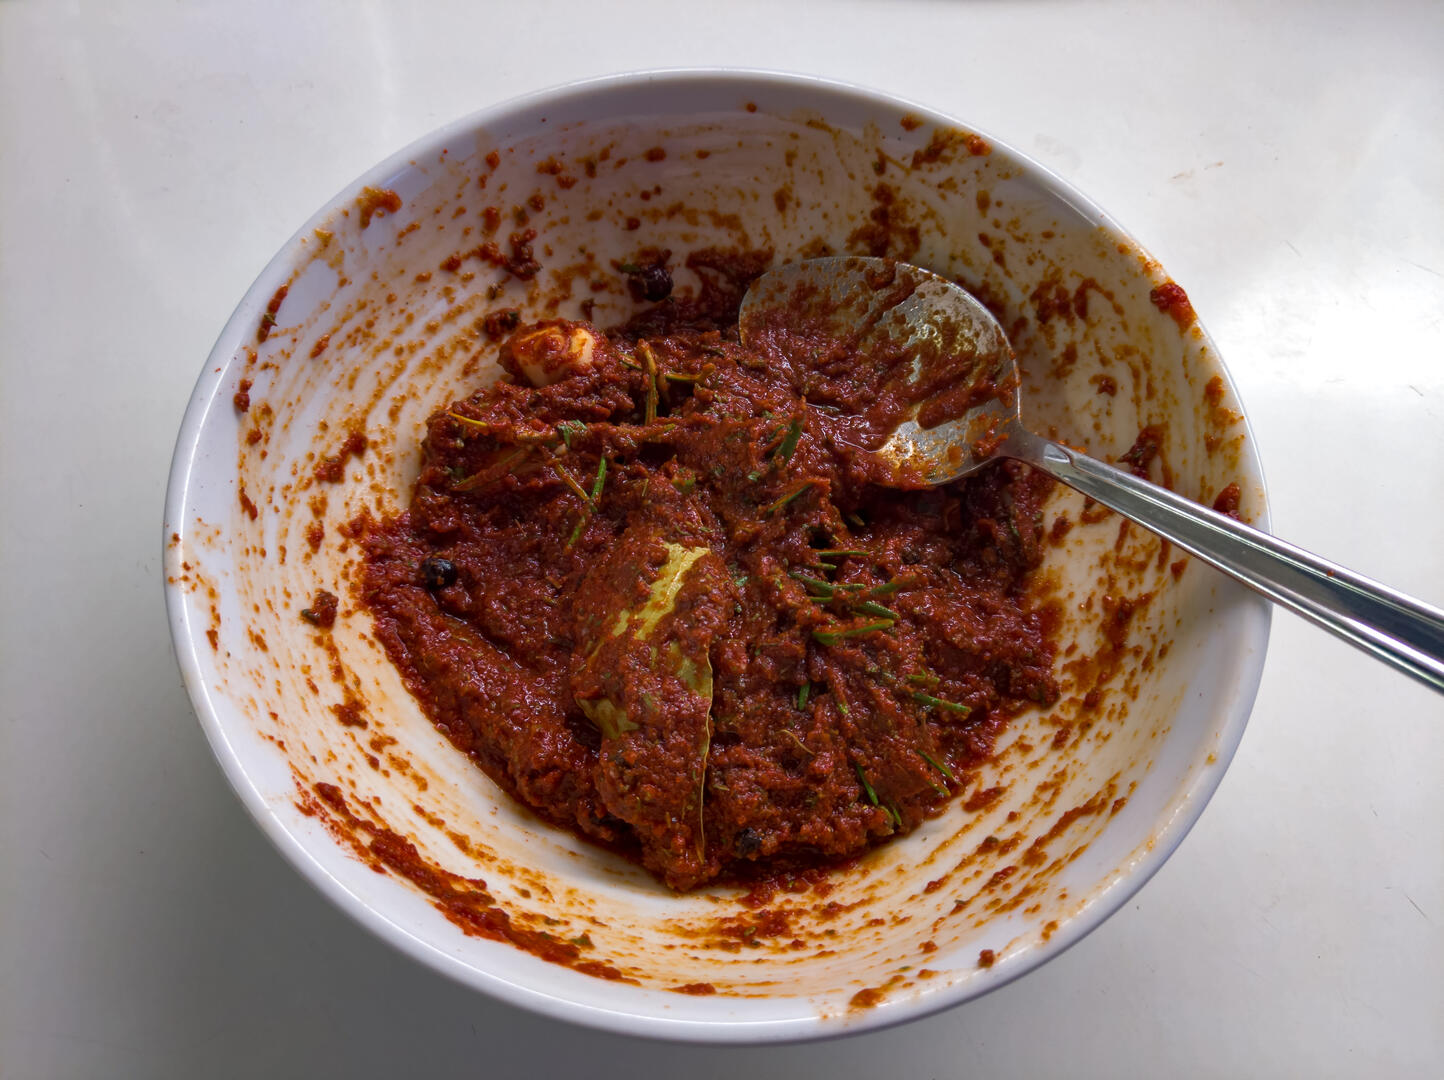
\includegraphics[width=0.5\textwidth]{goulash/IMG_20200202_095816.jpg}

            I pre-mix the spices with the tomato pur\'ee and the salt before adding them to the pot: mostly because I like how it looks and also to have something to do while the meat is browning.
	    }

	    \ingredients[16]{
            \SI{1}{\kilo\gram} & BEEF \\
            \SI{0.3}{\kilo\gram} & Onion \\
            1\,tsp & Thyme \\
            1\,tsp & Dry celery leaves \\
            1\,tsp & Summer savory (is apparently what it’s called) \\
            1\,tsp & Marjoram \\
            0.5\,tsp & Cumin \\
            1.5\,tsp & Caraway \\
            1\,large & Bay leaf or several small bay leaves \\
            idk some & Whole peppercorns \\
            7--10 & Juniper berries \\
            1.5\,tbsp & Paprika \\
            1\,sprig & Rosemary \\
            2\,cloves & Garlic \\
            1\,mTc & Salt! \\
            2\,tbsp & Tomato pur\'ee
        }

    \preparation{

        \step Clean and cut the meat into walnut-sized qubes. You don’t have to remove all fat and connective tissue, but the more you leave the longer it will take to render and soften.

%        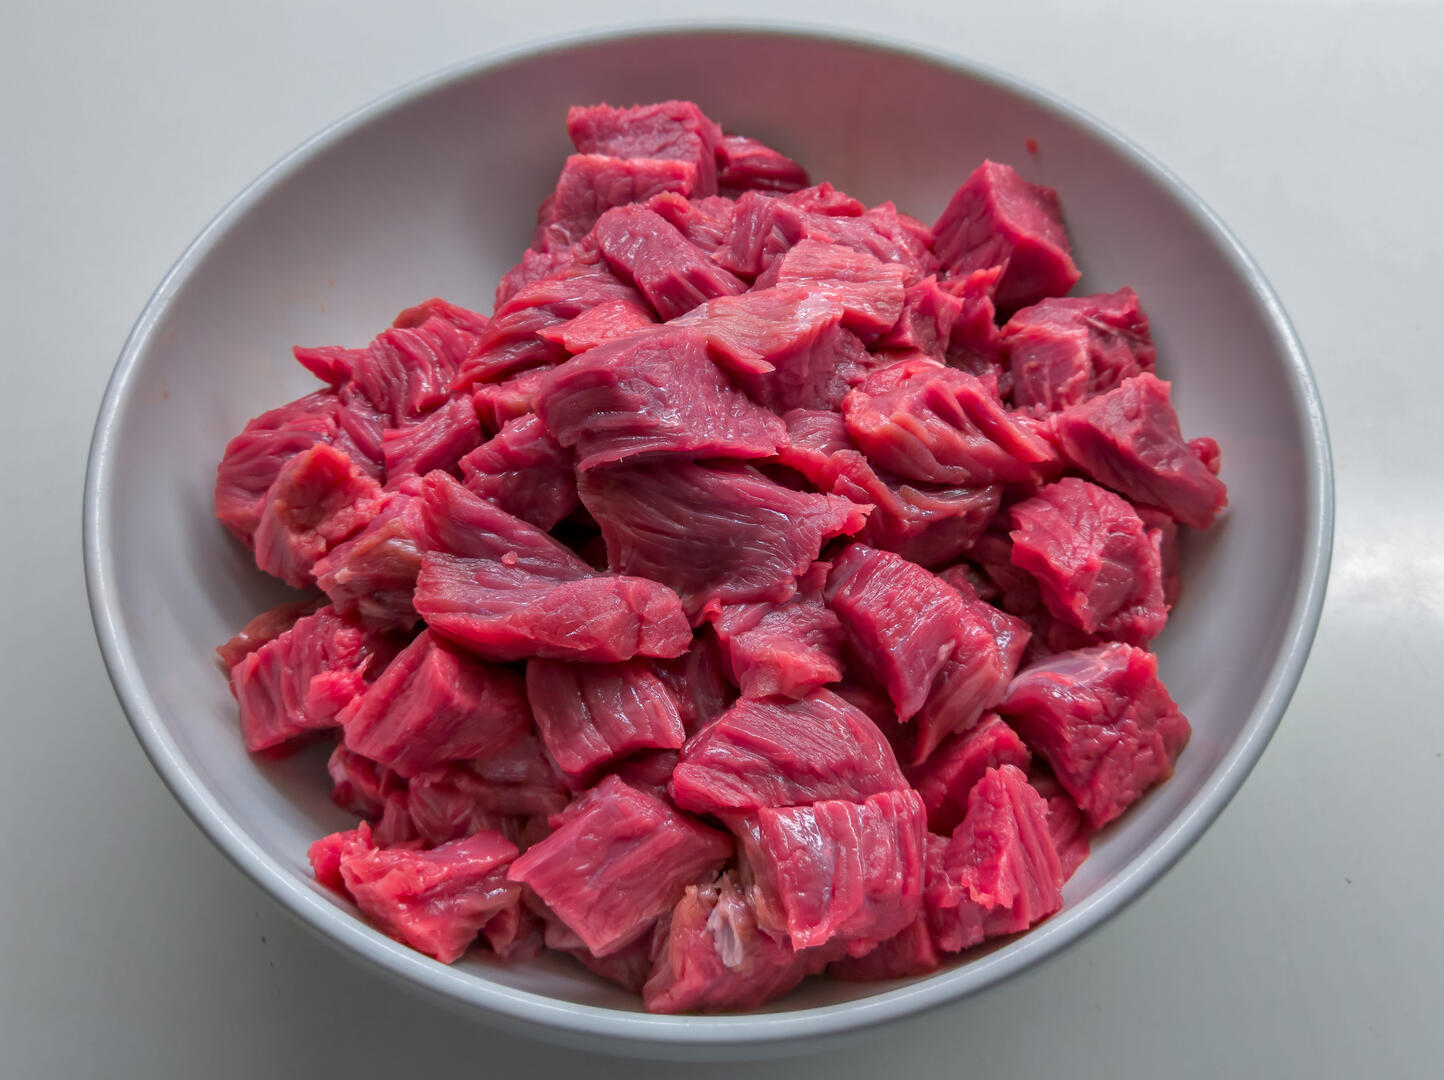
\includegraphics[width=0.53\textwidth]{goulash/IMG_20200202_091357.jpg}


        \step Slice the onions. The onions will ``melt'' while they cook, so you can chop them very roughly: small onions into quarters, larger onions lengthwise into 1 cm strips. Also, you’re cleaning and slicing like a kilogram of onions; you don’t wanna finely chop that many onions, do you?

%        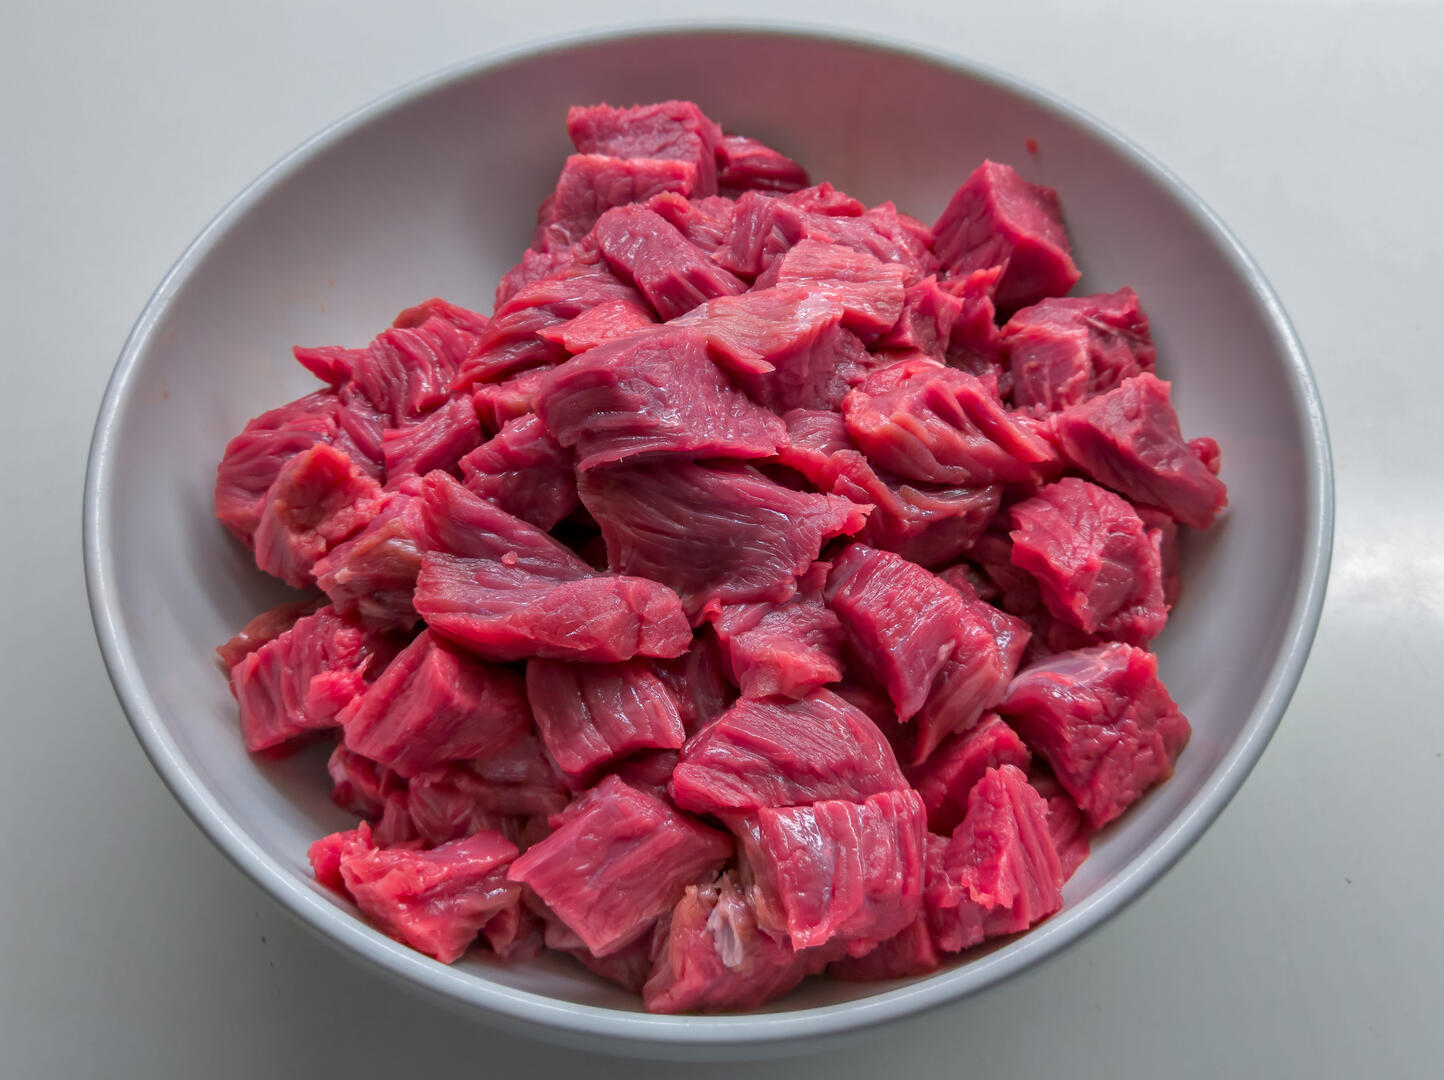
\includegraphics[width=0.5\textwidth]{goulash/IMG_20200202_091357.jpg}%
%        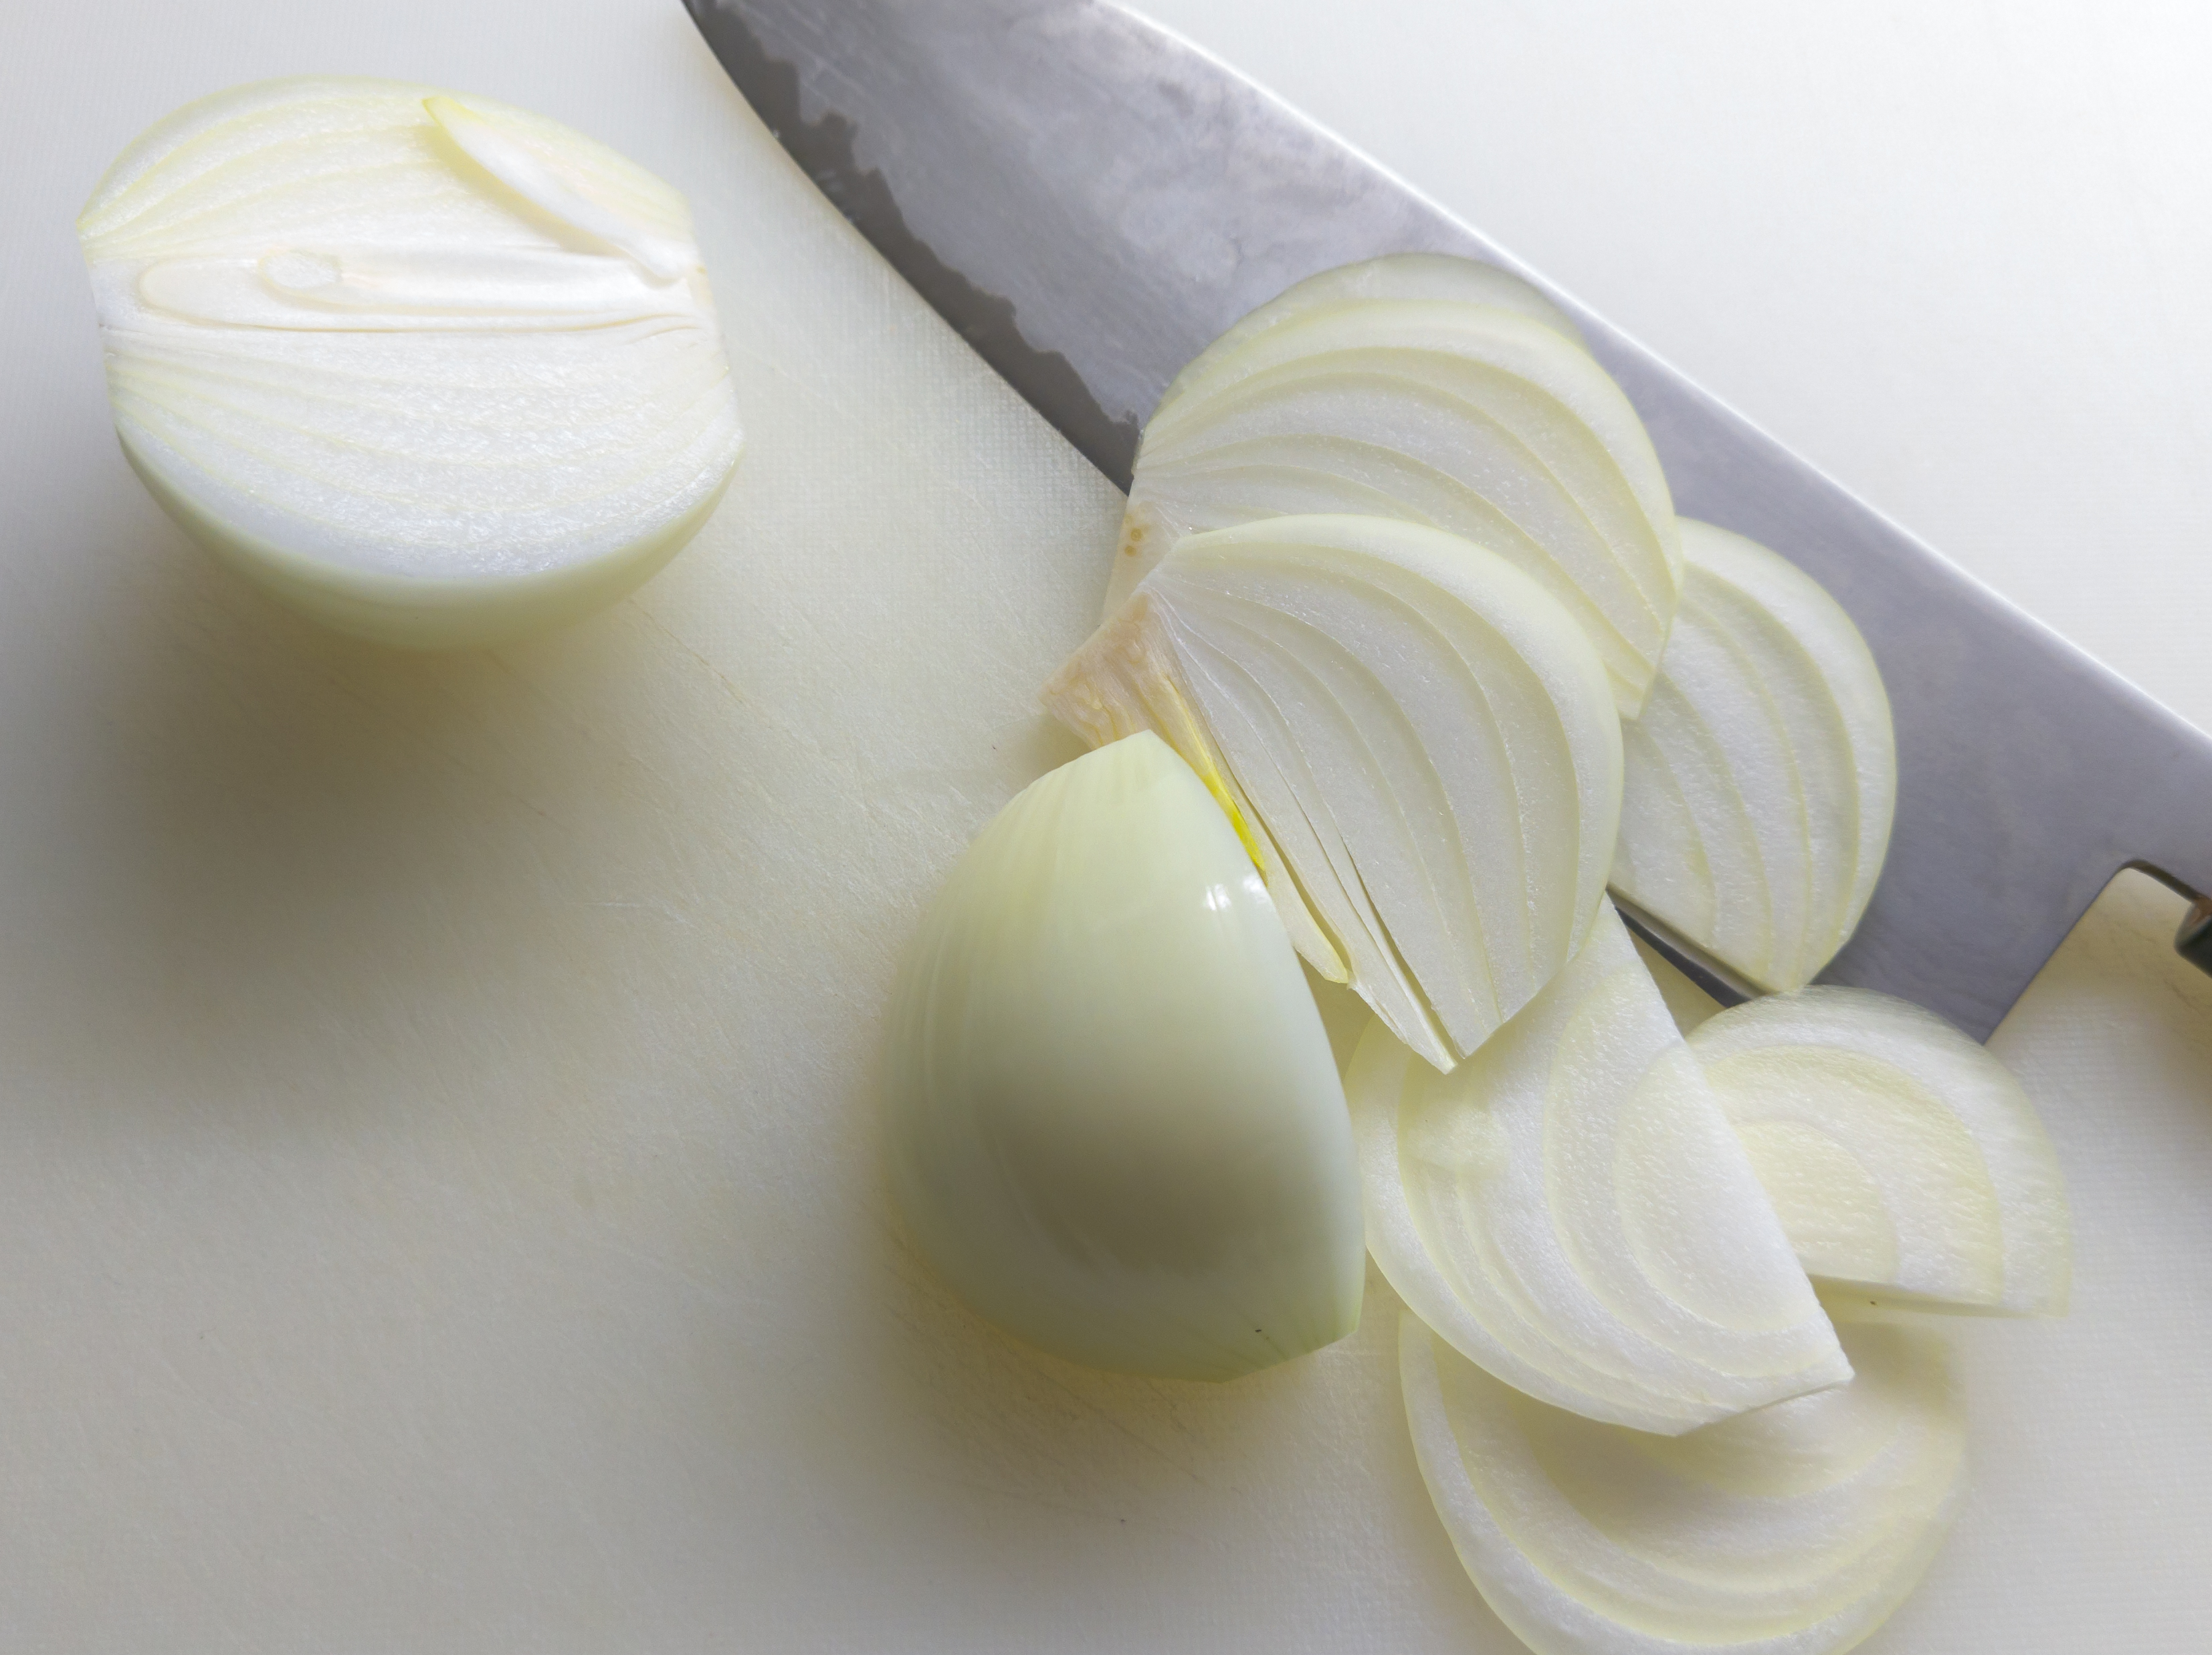
\includegraphics[width=0.5\textwidth]{goulash/IMG_20200202_091811.jpg}

%        \begin{wrapfigure}[11]{r}{0.51\textwidth}%
%            % \centering%
%            \hspace{-23pt}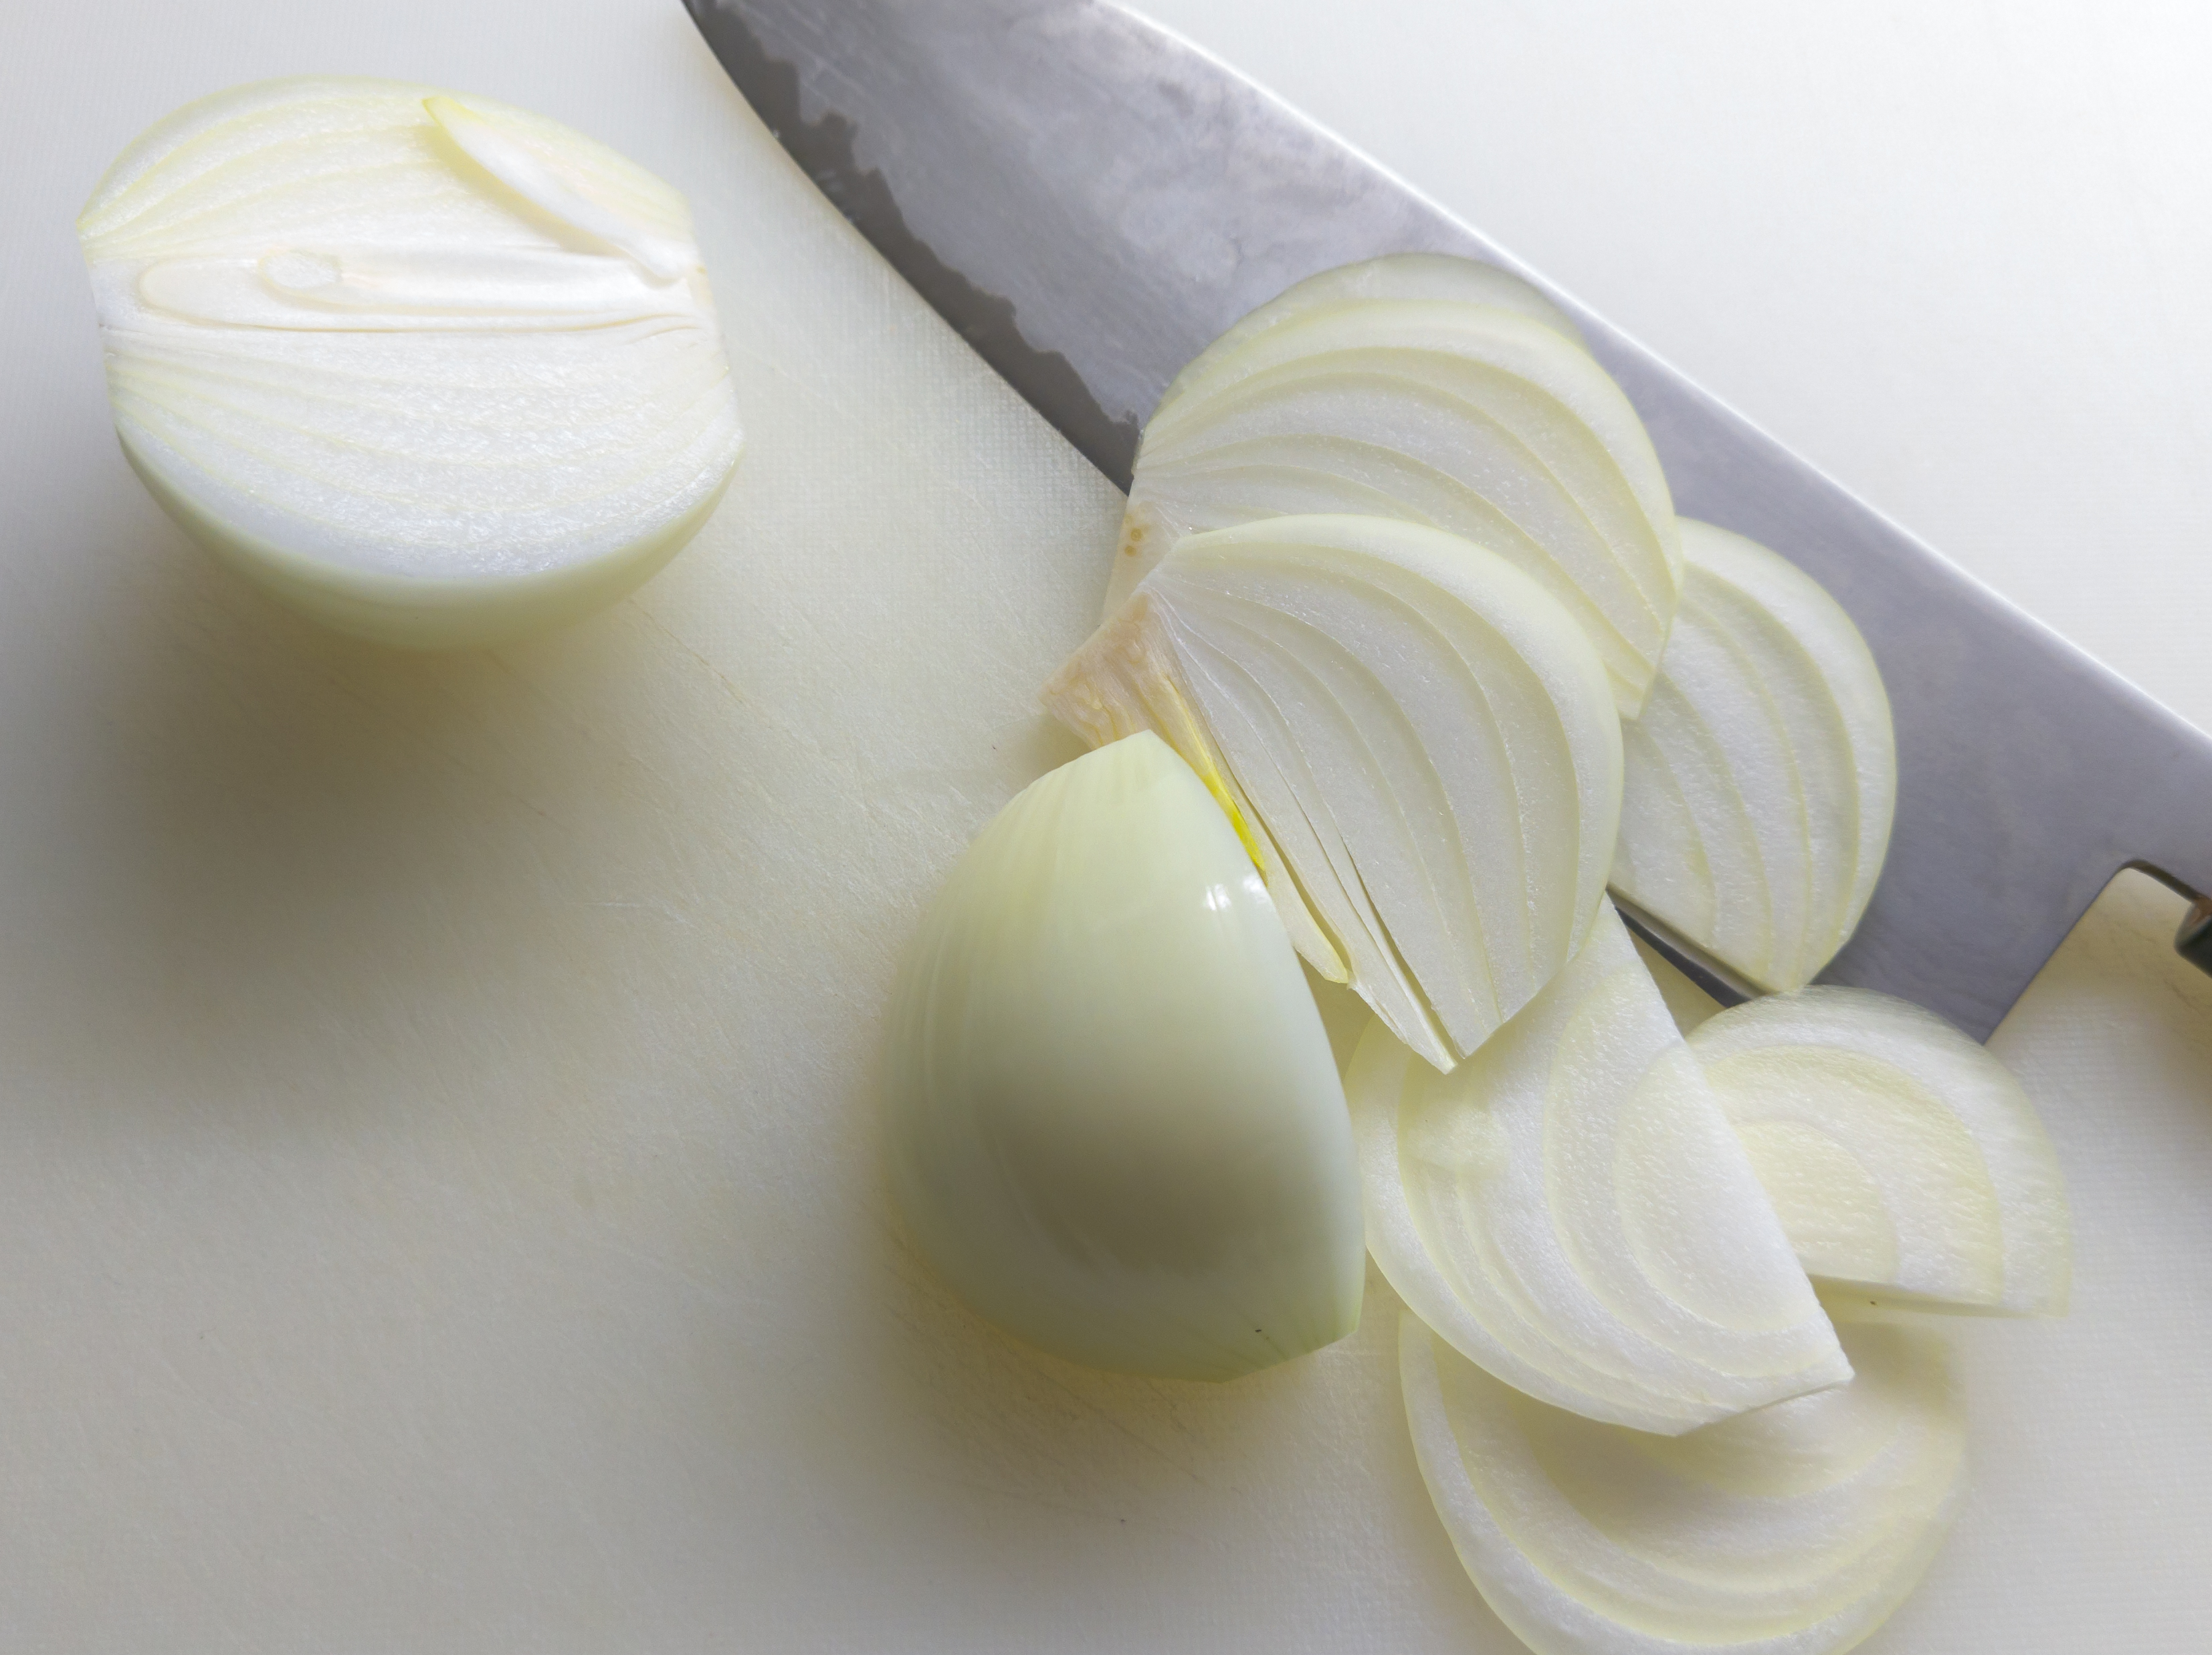
\includegraphics[width=0.5\textwidth]{goulash/IMG_20200202_091811.jpg}
%        \end{wrapfigure}

        \step Start saut\'eing the onions on high-mid heat on a bit of oil.

        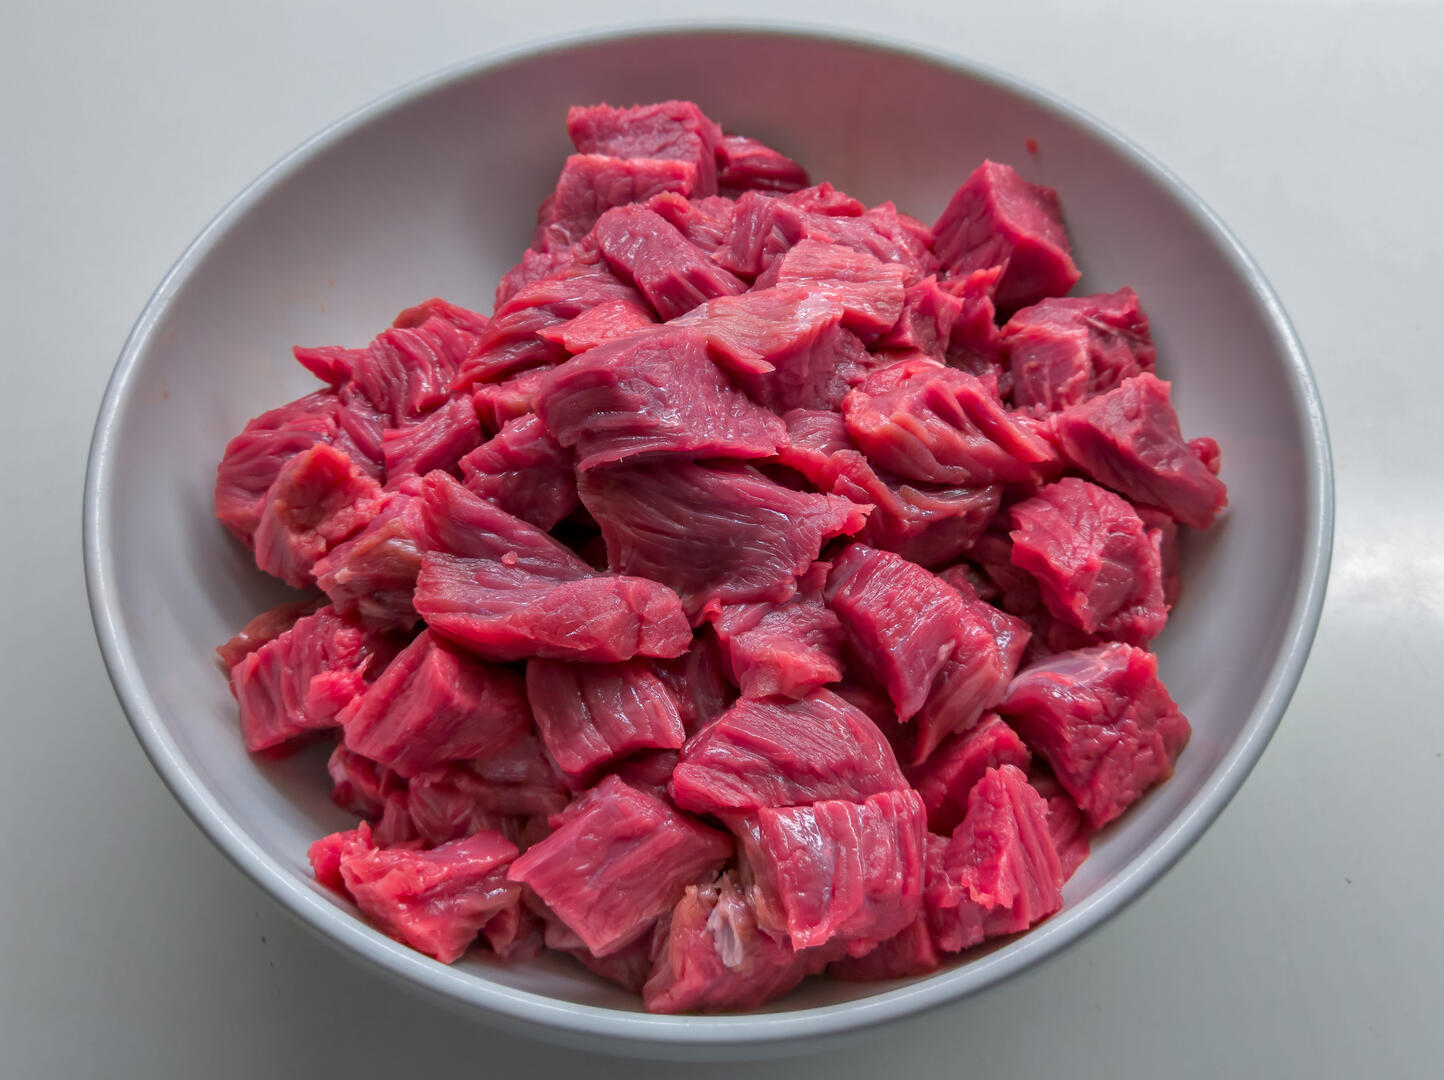
\includegraphics[width=0.5\textwidth]{goulash/IMG_20200202_091357.jpg}%
        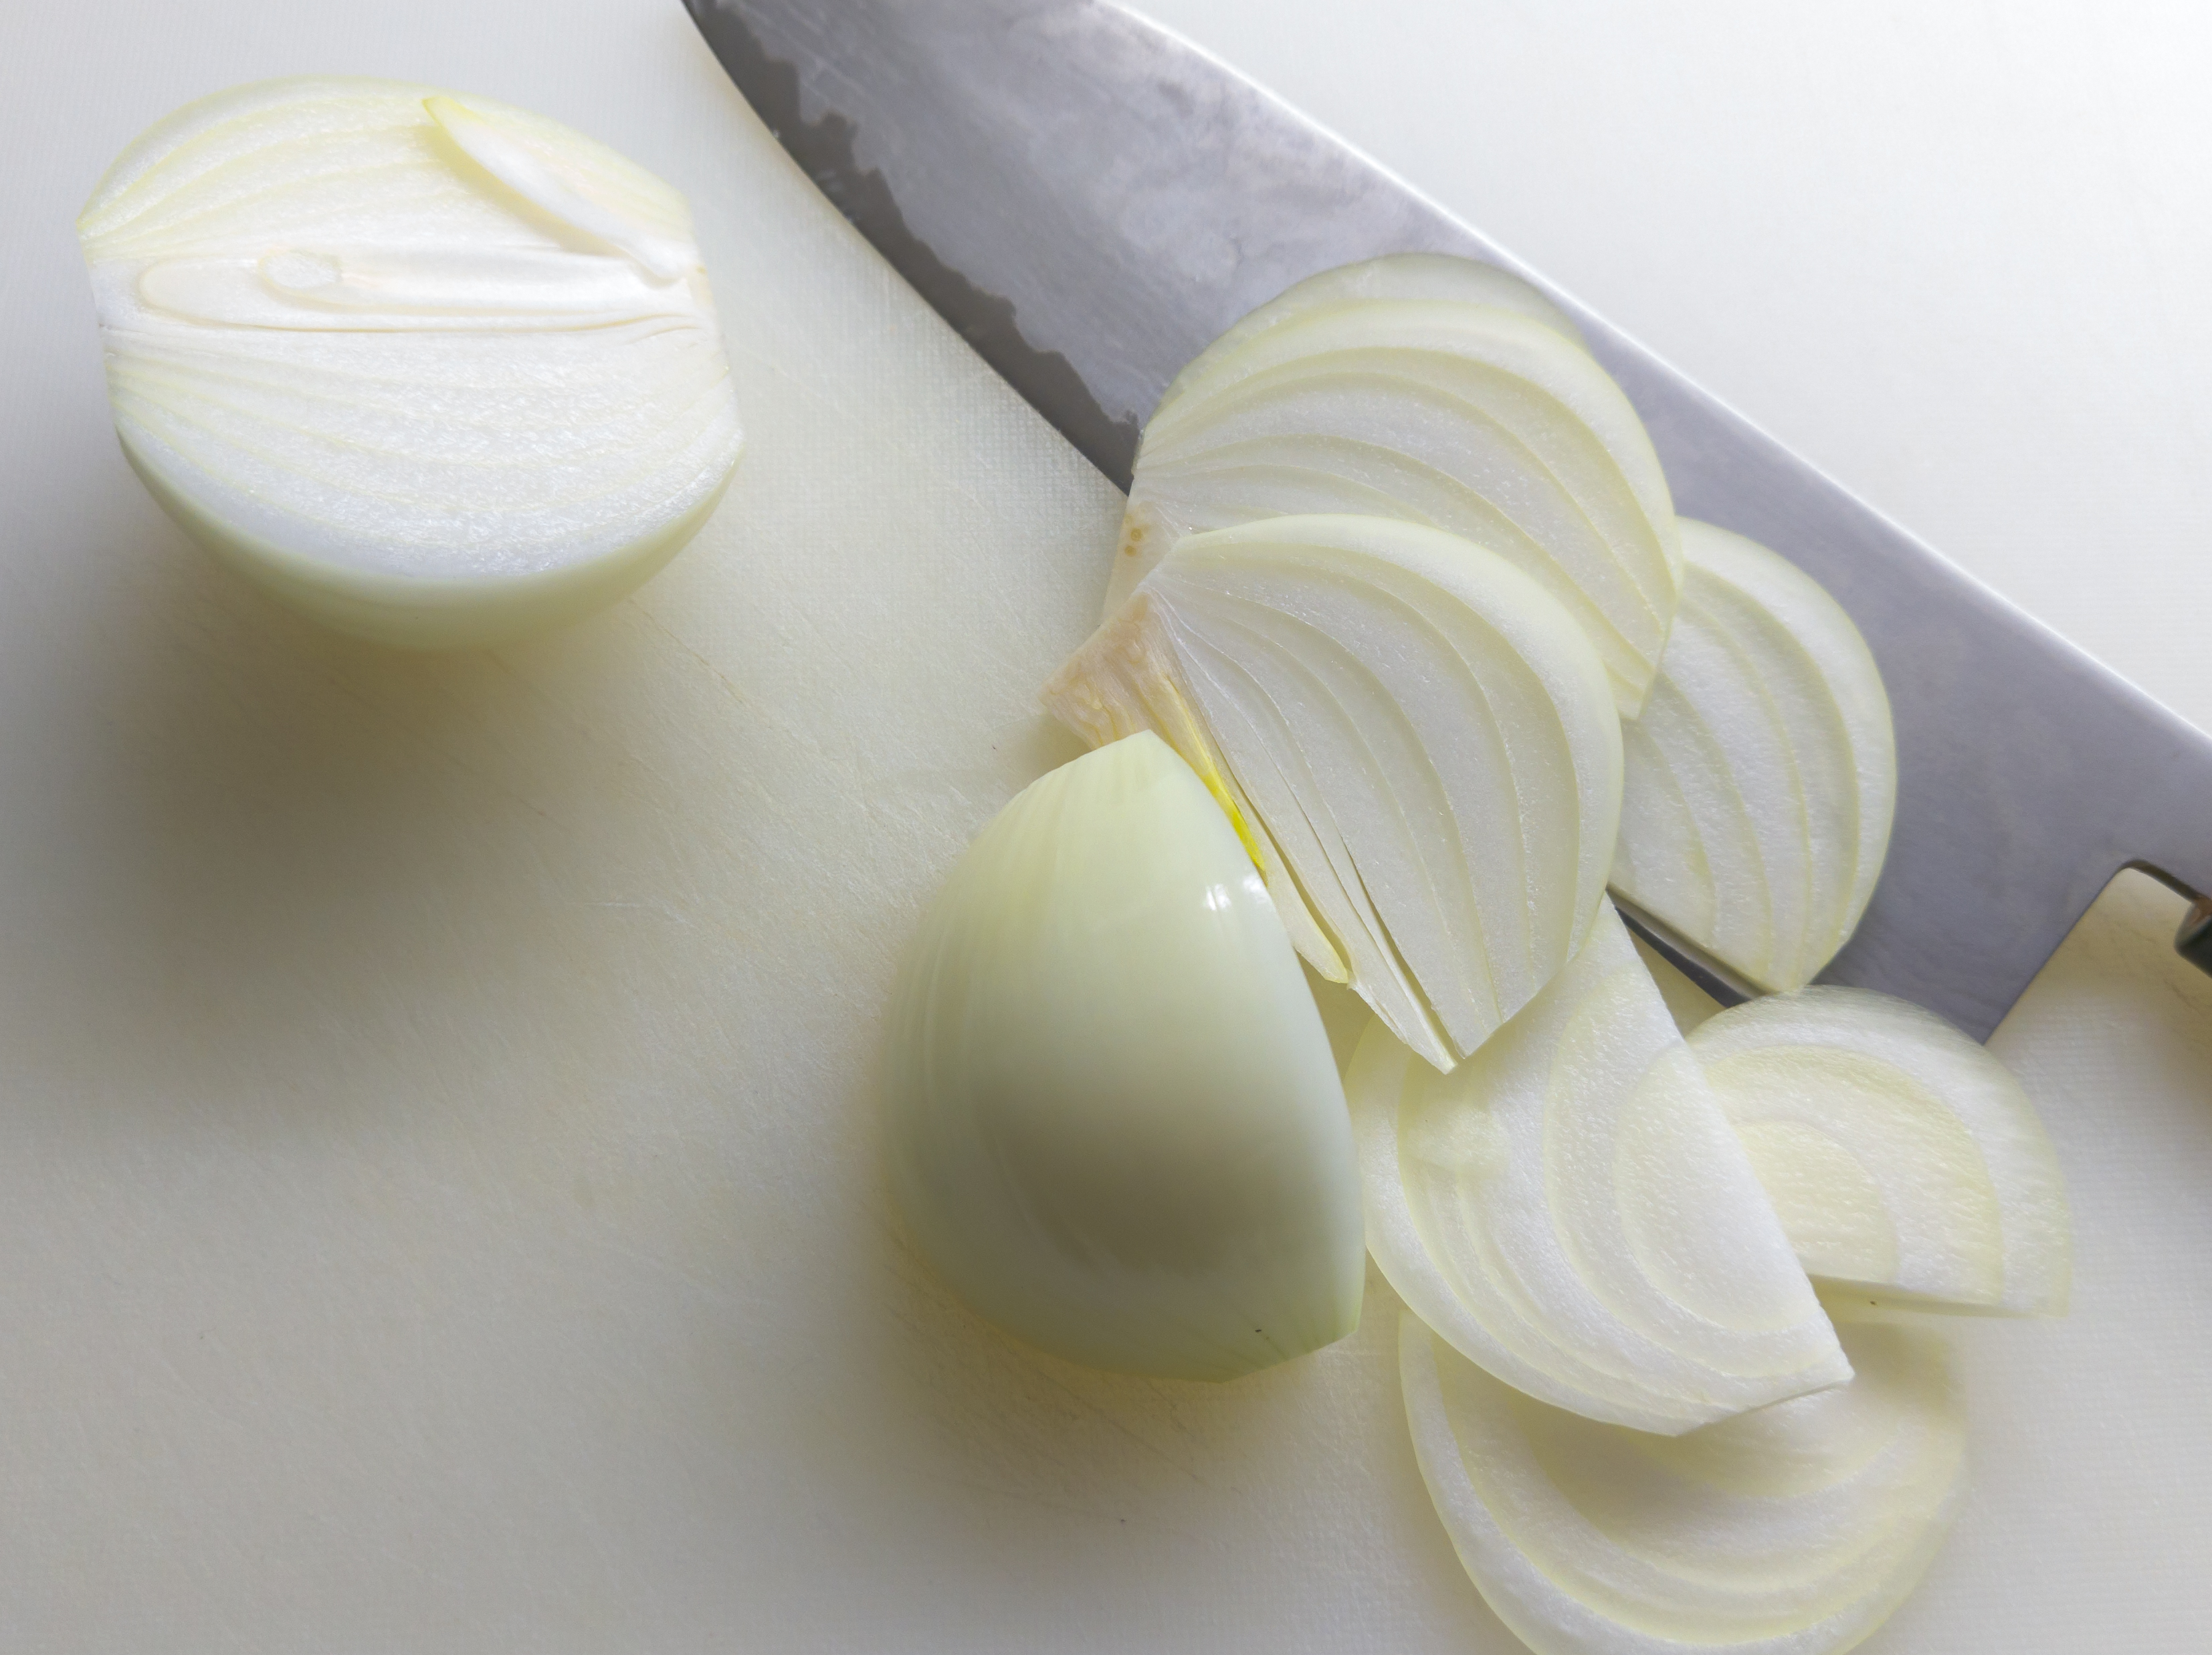
\includegraphics[width=0.5\textwidth]{goulash/IMG_20200202_091811.jpg}

%        \vspace{1em}

        \step When they start to brown add the meat. The meat will probably release a lot of liquid\footnote{ Normally, this effect, called ``crowding the pan,'' is bad as it can ruin the sear on a good steak, but in this case, we are going to stew the meat anyway, so it doesn’t change much.}. If that happens, raise the temperature and boil it off until it turns dark brown. This can take \textit{quite} a while. Otherwise, just brown the meat.

        \step Add wine and cook until it mostly boils off.

    	\vspace{1em}

        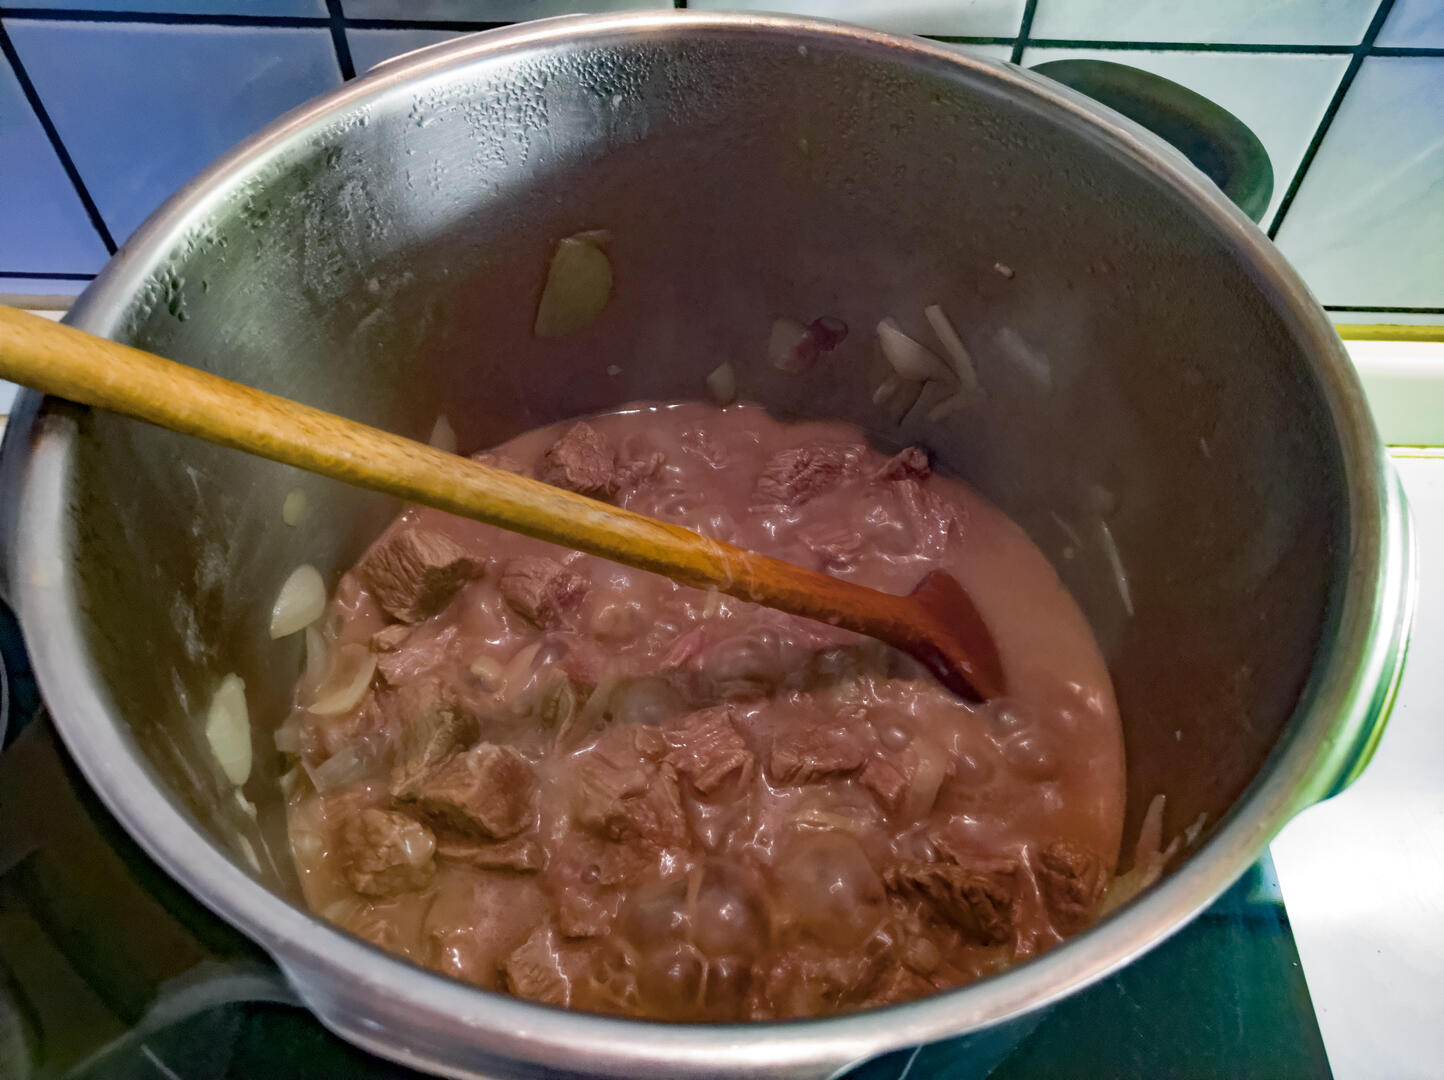
\includegraphics[width=0.5\textwidth]{goulash/IMG_20200202_095411.jpg}%
        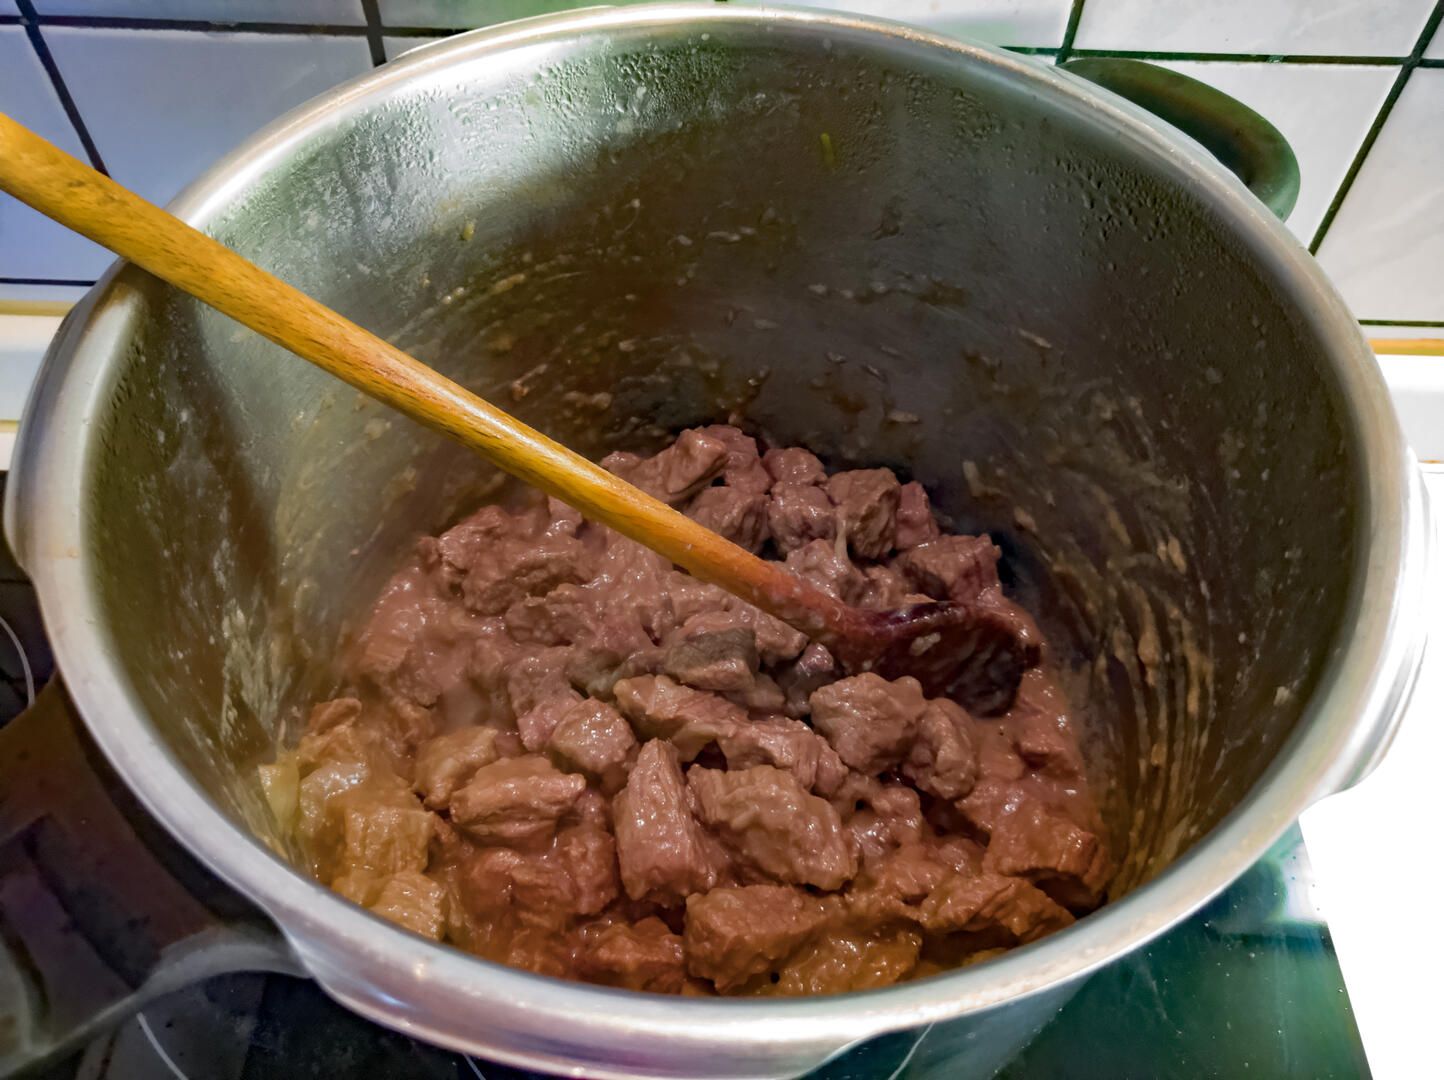
\includegraphics[width=0.5\textwidth]{goulash/IMG_20200202_101611.jpg}

        \step Add the spices with the salt and the tomato pur\'ee and add just enough water to cover everything.

        \step Keep simmering on low for at least 90 minutes; the longer the better. Keep adding water if too much boils off. If you’re using a pressure cooker you can shorten that time, but honestly, use the same time to get a better result.

        \step Serve. I like to have some nice bread with it, but gnocchi is also an option or some other pasta. Really, any starch works.
    }
\end{recipe}